\documentclass[a4paper,oneside,12pt]{extreport}
\usepackage[T2A,T1]{fontenc}
\usepackage[utf8]{inputenc}
\usepackage[english,russian]{babel}

\usepackage[left=30mm, right=15mm, top=20mm, bottom=20mm]{geometry}

\usepackage{microtype}
\sloppy

\usepackage{setspace}
\onehalfspacing

\usepackage{indentfirst}
\setlength{\parindent}{1.25cm}

\usepackage{titlesec}
\titleformat{\chapter}{\LARGE\bfseries}{\thechapter}{20pt}{\LARGE\bfseries}
\titleformat{\section}{\Large\bfseries}{\thesection}{20pt}{\Large\bfseries}

\titlespacing*{\chapter}{0pt}{0pt}{20pt}


\usepackage{wrapfig}
% \usepackage{float}

% \makeatletter
% \renewcommand{\fnum@figure}{Рисунок \thefigure}
% \makeatother


\usepackage{pgfplots}
\pgfplotsset{compat=newest}

\usepackage{listings}
\lstset{
	basicstyle=\footnotesize\ttfamily,
	keywordstyle=\color{blue},
	stringstyle=\color{red},
	commentstyle=\color{gray},
	numbers=left,
	numberstyle=\tiny,
	numbersep=5pt,
	frame=false,
	breaklines=true,
	breakatwhitespace=true,
}

\newcommand{\code}[1]{\texttt{#1}}

\usepackage{amsmath}
\usepackage{amssymb}

\usepackage{tikz}
\usetikzlibrary{arrows}
\usetikzlibrary{shapes}

\usepackage{booktabs}
\usepackage{array}
\usepackage{adjustbox}

\usepackage{enumerate}

\usepackage[unicode]{hyperref}
\hypersetup{hidelinks}

\makeatletter
\def\vhrulefill#1{\leavevmode\leaders\hrule\@height#1\hfill \kern\z@}
\makeatother


\usepackage{csvsimple}

\usepackage{caption}
\usepackage[justification=centering]{caption}
% \captionsetup{justification=centering}


\def\lab{7}
\def\topic{Расстояние Левенштейна и Дамерау-Левенштейна}
\def\topic{Алгоритмы умножения матриц}
\def\topic{Алгоритмы сортировки}
\def\topic{Параллельные вычисления}
\def\topic{Многопоточная реализация конвейера}
\def\topic{Муравьиный алгоритм и полный перебор}
\def\topic{Поиск в словаре}


\begin{document}

\begin{titlepage}
	\centering
	\large
	
	\begin{wrapfigure}[7]{l}{0.14\linewidth}
		\vspace{5mm}
		\hspace{-5.8mm}
		
\includegraphics[width=0.93\linewidth]{../../report/common/bmstu-logo}
	\end{wrapfigure}
	{\singlespacing \footnotesize \bfseries Министерство науки и высшего образования Российской Федерации\\Федеральное государственное бюджетное образовательное учреждение\\высшего образования\\<<Московский государственный технический университет\\имени Н.~Э.~Баумана\\ (национальный исследовательский университет)>>\\(МГТУ им. Н.~Э.~Баумана)\\}

	\vspace{-2.2mm}
	\vhrulefill{0.9mm}\\
	\vspace{-7.5mm}
	\vhrulefill{0.2mm}\\
	\vspace{2mm}
	
	{\doublespacing \normalsize \raggedright ФАКУЛЬТЕТ \hspace{25mm} «Информатика и системы управления»\\
	КАФЕДРА \hspace{5mm} «Программное обеспечение ЭВМ и информационные технологии»\\}

	\vspace{30mm}
	
	\textbf{ОТЧЕТ}\\
	По контрольной работе № 1\\
	По курсу: <<Анализ алгоритмов>>\\
	Тема: <<\topic>>\\

	\vspace{60mm}

	\hspace{70mm} Студент:      \hfill Ле Ни Куанг\\
	\hspace{70mm} Группа:       \hfill ИУ7и-56Б\\
	\hspace{70mm} Преподаватель:\hfill Волкова Л. Л.\\
								\hfill Строганов Ю. В.\\
	% {\raggedright \hspace{70mm} Оценка: \hfill \hrulefill\\}

	\vfill
	
	Москва\\
	\the\year
\end{titlepage}

\setcounter{page}{2}
\tableofcontents

\chapter*{Введение}
\addcontentsline{toc}{chapter}{Введение}


Умножение матриц - одна из основных операций над матрицами.
Матрица, получаемая в результате операции умножения, называется
произведением матриц.\\


\textbf{Целью работы:} изучение алгоритмов умножения матриц. В данной
лабораторной работе рассматривается стандартный алгоритм умножения
матриц, алгоритм Винограда и модифицированный алгоритм Винограда.
Также требуется изучить рассчет сложности алгоритмов, получить навыки
в улучшении алгоритмов.
\\

\textbf{Задачи работы:}

\begin{enumerate}
    \setlength{\itemsep}{0em}
    \item изучить алгоритмы умножения матриц: стандартный и алгоритм Винограда,
    оптимизировать алгоритм Винограда.
    \item дать теоретическую оценку алгоритмы (трудоемкость).
    \item реализовать три алгоритма умножения матриц.
    \item сравнить алгоритмы умножения матриц.
\end{enumerate}

\chapter{Аналитический раздел}
\label{cha:analysis}

В данном разделе представлены теоретические сведения о
алгоритмах поиска в словаре.

\section{Алгоритм полного перебора}

Алгоритм перебирает ключи словаря, пока не будет найден искомый ключ.
Возможно (N + 1) случаев: ключ не найден и N возможных случаев расположения ключа в словаре.
Лучший случай: за одно сравнение ключ найден в начале словаря.
Худших случаев два: за N сравнений либо элемент не найден, либо ключ найден на последнем сравнении.
Трудоемкость в среднем:
\begin{equation}
    \sum\limits_{i\in\Omega} p_i\cdot f_i =
    k_0+k_1(1+\frac{N}{2}-\frac{1}{N+1})
\end{equation}


\section{Алгоритм двоичного поиска}

Алгоритм требует ключи словаря отсортированы.
При двоичном поиске обход можно представить деревом, поэтому трудоемкость в худшем случае составит $log_2N$
(в худшем случае нужно спуститься по двоичному дереву от корня до листа).
Скорость роста функции $log_2N$ меньше чем у N.


\section{Алгоритм частотного анализа}

Алгоритм на вход получает словарь и на его основе составляется частотный анализ. По полученным значениям словарь разбивается на сегменты так, что все элементы с одинаковым первым элементом оказываются в одном сегменте. 

Сегменты упорядочиваются по значению частотной характеристики так, чтобы к элементы с наибольшей частотной характеристикой был самый быстрый доступ. 

Далее каждый сегмент упорядочивается по значению. Это необходимо для реализации бинарного поиска, который обеспечит эффективный поиск в сегменте при сложности $O(\log n)$.

Таким образом, сначала выбирается нужный сегмент, а затем в нем проводится бинарный поиск нужного элемента. Средняя трудоёмкость при длине алфавита $M$ может быть рассчитана по формуле \ref{eq:tfa}. 

\begin{equation} \label{eq:tfa}
	\sum\limits_{i\in[1, M]} (f_{\text{выбор i-го сегмента}}+f_{\text{поиск в i-ом сегменте}}) \cdot p_i
\end{equation}


\section{Описание словаря}

Словарь представляет собой набор информации о 1000 распространенных криптовалютах на 24.01.21.
Запись словаря, реализованная на данной работе, имеет вид
( Rank: int, Name: string, Symbol: string, Market Cap: int64, Price: float32 ).
Поиск по полю Name.

\section{Вывод}
В данном разделе были описаны два алгоритма и способ оптимизации для поиска в словаре.
Так же был рассмотрен описание словаря.
\chapter{Конструкторский раздел}
\label{cha:design}

В данном разделе будет приведено описание схем алгоритмов
сортировка пузырьком, сортировка вставками, сортировка слиянием
и вычислены их трудоемкости.

\section{Разработка алгоритмов}

На рисунках \ref{fig:2.1}, \ref{fig:2.2}, \ref{fig:2.3} показаны схемы алгоритмов сортировки.


% \pagebreak
\subsection{Сортировкa пузырьком}

\begin{figure}[h]
    \centering
    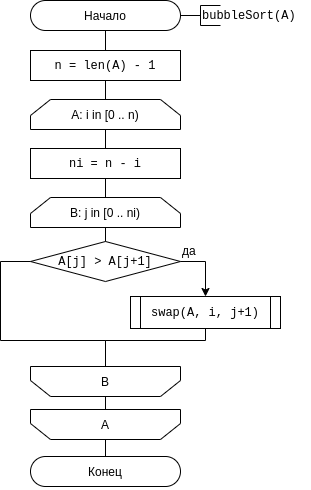
\includegraphics[width=0.48\textwidth]{3/inc/d1.png}
    \caption{Схема алгоритма сортировкa пузырьком}
    \label{fig:2.1}
\end{figure}


\newpage
\subsection{Сортировкa вставками}

\begin{figure}[h!]
    \centering
    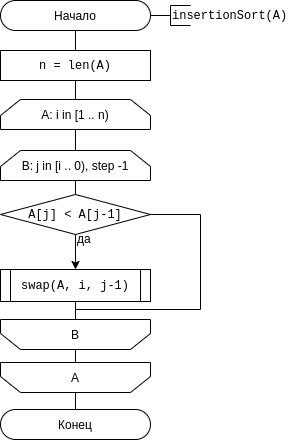
\includegraphics[width=0.52\textwidth]{3/inc/d2.png}
    \caption{Схема алгоритма сортировкa вставками}
    \label{fig:2.2}
\end{figure}

\newpage
\subsection{Сортировкa слиянием}

\begin{figure}[h!]
    \centering
    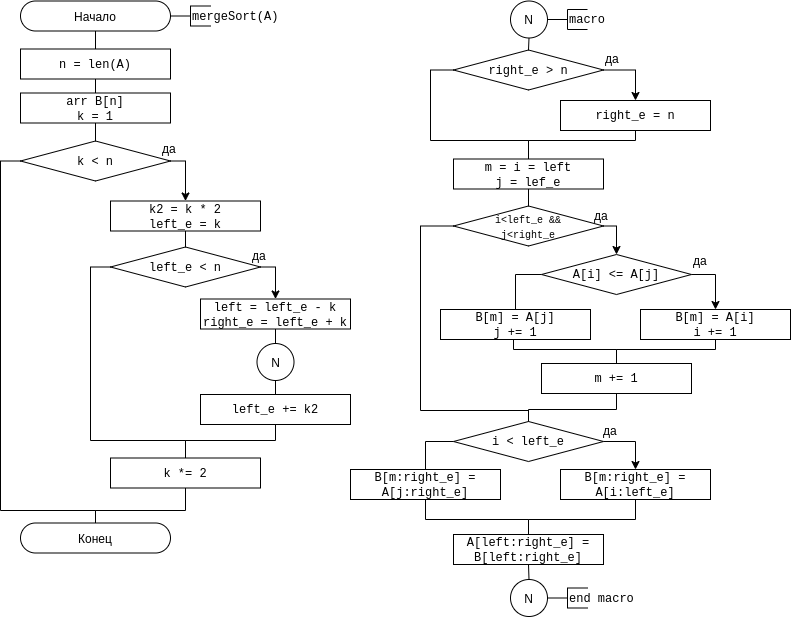
\includegraphics[width=1\textwidth]{3/inc/d3.png}
    \caption{Схема алгоритма сортировкa слиянием}
    \label{fig:2.3}
\end{figure}


\clearpage
\section{Оценка трудоемкости}

Применить формулы \ref{eq:1.1} и \ref{eq:1.2}.
Предположим, что сложность $swap()$ равна 5, сложность $len()$ равна n.

\subsection{Сортировкa пузырьком}


\begin{tabular}{|c|c|}
    \hline
    $F_{if}$        & $\left\{
        \begin{array}{ll}
            4, \hspace{0.5cm} $л.с.$\\
            9, \hspace{0.5cm} $х.с.$\\
        \end{array}
        \right.$ \\\hline\hline
    $F_{forA}$      & $\left\{
        \begin{array}{ll}
            4n + 6 \cdot \dfrac{(n-2)(n-1)}{2} = 3n^2 - 5n + 6, \hspace{0.5cm} $л.с.$\\
            4n + 11 \cdot \dfrac{(n-2)(n-1)}{2} = 5.5n^2 - 12.5n + 11, \hspace{0.5cm} $х.с.$\\
        \end{array}
        \right.$ \\\hline\hline
    $F_{bubble}$    & $\left\{
        \begin{array}{ll}
            3n^2 - 4n + 10, \hspace{0.5cm} $л.с.$\\
            5.5n^2 - 11.5n + 15, \hspace{0.5cm} $х.с.$\\
        \end{array}
        \right.$ \\\hline
\end{tabular}


\subsection{Сортировкa вставками}

\begin{tabular}{|c|c|}
    \hline
    $F_{if}$        & $\left\{
        \begin{array}{ll}
            4, \hspace{0.5cm} $л.с.$\\
            9, \hspace{0.5cm} $х.с.$\\
        \end{array}
        \right.$ \\\hline\hline
    $F_{forA}$      & $\left\{
        \begin{array}{ll}
            2n + 6 \cdot \dfrac{(n-2)(n-1)}{2} = 3n^2 - 7n + 6, \hspace{0.5cm} $л.с.$\\
            2n + 11 \cdot \dfrac{(n-2)(n-1)}{2} = 5.5n^2 - 14.5n + 11, \hspace{0.5cm} $х.с.$\\
        \end{array}
        \right.$ \\\hline\hline
    $F_{insert}$    & $\left\{
        \begin{array}{ll}
            3n^2 - 6n + 9, \hspace{0.5cm} $л.с.$\\
            5.5n^2 - 13.5n + 14, \hspace{0.5cm} $х.с.$\\
        \end{array}
        \right.$ \\\hline
\end{tabular}


\subsection{Сортировкa слиянием}

В любом случае сложность сортировки слиянием $nlog_2n$ \cite{b4}.


\section{Вывод}
В данном разделе было приведено описание схем алгоритмов и вычислены их трудоемкости.

\chapter{Технологический раздел}
\label{cha:impl}

% \section{Требования к программному обеспечению}


\section{Средства реализации}

Язык программирования: Python (IPython)

Библиотеки: unittest, timeit, matplotlib, ...

Редактор: Jupyter-Lab

Я использую эти инструменты потому, что они мощные, широко
используемые и знакомые мне.


\section{Листинг кода}


\lstinputlisting[
    language=python,linerange={0-9},
    caption=Сортировка пузырьком
    ]{3/inc/code.py}

\vbox{}

\lstinputlisting[
    language=python,linerange={10-19},
    caption=Сортировка вставками
    ]{3/inc/code.py}

\pagebreak
\lstinputlisting[
    language=python,linerange={20-80},
    caption=Сортировка слиянием
    ]{3/inc/code.py}

\pagebreak
\section{Описание тестирования}

В таблице \ref{tabular:func_test} приведен функциональные тесты
для алгоритмов сортировки.

\def\arraystretch{1.2}
\setlength\tabcolsep{1cm}

\begin{table}[h]
    \centering
    \csvreader[tabular=|c|c|,
        no head,
        table head=\hline \bfseries Массив & \bfseries Результат \\\hline,
        late after line=\\\hline]
        {3/inc/func_test.csv}{}{ \csvcoli & \csvcolii}
    \caption{\label{tabular:func_test} Функциональные тесты}
\end{table}

\setlength\tabcolsep{0.5cm}

\section{Вывод}

В этом разделе было рассмотрено код программы и описание тестирования.
\chapter{Экспериментальный раздел}
\label{cha:research}

\section{Примеры работы}
На рисунке \ref{fig:4.1} приведен пример работы программы.

\begin{figure}[h]
    \centering
    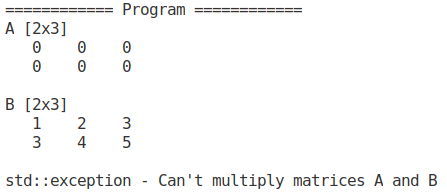
\includegraphics[width=0.6\textwidth]{2/inc/e1.png}
    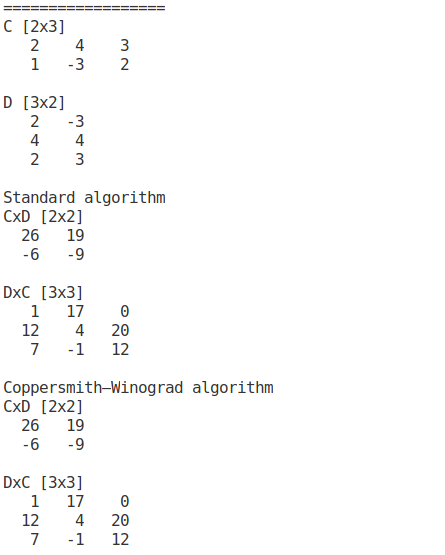
\includegraphics[width=0.6\textwidth]{2/inc/e2.png}
    \caption{Примеры работы алгоритмов умножения матриц}
    \label{fig:4.1}
\end{figure}


\pagebreak
\section{Результаты тестирования}

На рисунке \ref{fig:4.2} приведен результат теста с использованием фреймворка google test.

\begin{figure}[h]
    \centering
    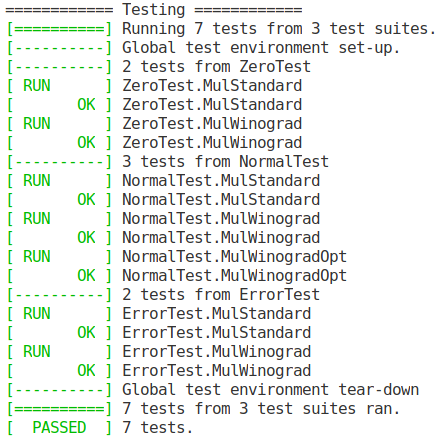
\includegraphics[width=0.6\textwidth]{2/inc/test.png}
    \caption{Примеры работы алгоритмов умножения матриц}
    \label{fig:4.2}
\end{figure}


% \section{Постановка эксперимента по замеру времени}
\section{Сравнение времени работы}

В таблице \ref{tabular:benchmark} приведены замеры времени
работы алгоритмов умножения матриц на квадратных матрицах,
на основе них построены графики \ref{fig:4.3} и \ref{fig:4.4}.

%  приведен функциональные тесты для алгоритмов
% вычисления расстояния Левенштейна и Дамерау — Левенштейна.


\def\arraystretch{1.2}
% \setlength\tabcolsep{0.2cm}

\pagebreak
\begin{table}[h]
    \centering
    \csvreader[tabular=|c|c|c|c|,
        table head=\hline
        \bfseries Размер
        & \bfseries Стандартный
        & \bfseries Винограда
        & \bfseries Винограда(о)
        \\\hline,
        late after line=\\\hline]
        {2/inc/benchmark1.csv}{}
    { \csvcoli & \csvcolii & \csvcoliii & \csvcoliv}
    \csvreader[tabular=|c|c|c|c|,
        table head=\hline
        \bfseries Размер
        & \bfseries Стандартный
        & \bfseries Винограда
        & \bfseries Винограда(о)
        \\\hline,
        late after line=\\\hline]
        {2/inc/benchmark2.csv}{}
    { \csvcoli & \csvcolii & \csvcoliii & \csvcoliv}
    % \csvautotabular{2/inc/benchmark2.csv}
    \caption{\label{tabular:benchmark} Времени работы (ns)}
\end{table}

% \clearpage
\pagebreak
\begin{figure}[!h]
    \centering
    \begin{tikzpicture}
        \begin{axis}[
            scale=1.4,
            axis lines=left,
            xlabel=Размер матрицы,
            ylabel={Время, нс},
            legend pos=north west,
            xmajorgrids=true,
            ymajorgrids=true
        ]
            \addplot table[x=n,y=t1,col sep=comma] {2/inc/benchmark1.csv};
            \addplot table[x=n,y=t2,col sep=comma] {2/inc/benchmark1.csv};
            \addplot table[x=n,y=t3,col sep=comma] {2/inc/benchmark1.csv};
            \legend{Стандартный, Винограда, Винограда(о)}
        \end{axis}
    \end{tikzpicture}
    \caption{Зависимость времени работы алгоритмов умножения матриц от размеры матрицы (при четном размере)}
    \label{fig:4.3}
\end{figure}


\begin{figure}[!h]
    \centering
    \begin{tikzpicture}
        \begin{axis}[
            scale=1.4,
            axis lines=left,
            xlabel=Размер матрицы,
            ylabel={Время, нс},
            legend pos=north west,
            xmajorgrids=true,
            ymajorgrids=true
        ]
            \addplot table[x=n,y=t1,col sep=comma] {2/inc/benchmark2.csv};
            \addplot table[x=n,y=t2,col sep=comma] {2/inc/benchmark2.csv};
            \addplot table[x=n,y=t3,col sep=comma] {2/inc/benchmark2.csv};
            \legend{Стандартный, Винограда, Винограда(о)}
        \end{axis}
    \end{tikzpicture}
    \caption{Зависимость времени работы алгоритмов умножения матриц от размеры матрицы (при нечетном размере)}
    \label{fig:4.4}
\end{figure}

% \section{Сравнительный анализ на материале экспериментальных данных}
% эксперименты+выводы

\section{Вывод}

Из графики, очевидно, что алгоритм Винограда с оптимизацией самый быстрый,
на матрицах размером 800x800 работает примерно на 20\% (15-25\% зависит от m четное или нечетное)
быстрее стандартный алгоритм.

\chapter*{Заключение}
\addcontentsline{toc}{chapter}{Заключение}

В ходе лабораторной работы было проведено сравнение трех алгоритмов сортировки:
сортировка пузырьком, сортировка вставками и сортировка слиянием.
Были сделаны следующие выводы:

\begin{itemize}
    \item сортировка слиянием на порядок быстрее сортировки пузырьком и
    вставками (использует дополнительную O(n) память);
    \item сортировка вставками быстрее сортировки пузырьком (без флаг)
    во всех случаях;
    \item сортировка вставками самый быстрый для почти отсортирован массив;
    \item на массив длины 1000, сортировка слиянием в 30 раз быстрее сортировки
    пузырьком и в 23 раз быстрее сортировки вставками по сравнению среднее времени работы.
\end{itemize}

\addcontentsline{toc}{chapter}{Литература}
\bibliographystyle{ugost2008}


\begin{thebibliography}{8}

    \bibitem{b1}
    Кнут Д. Э. Искусство программирования. Том 3. Сортировка и поиск = The Art of Computer Programming. Volume 3. Sorting and Searching
    / под ред. В. Т. Тертышного (гл. 5) и И. В. Красикова (гл. 6). — 2-е изд. — Москва: Вильямс, 2007. — Т. 3. — 832 с.

    \bibitem{b2}
    Томас Х. Кормен, Чарльз И. Лейзерсон, Рональд Л. Ривест, Клиффорд Штайн.
    Алгоритмы: построение и анализ = Introduction to algorithms.
    — 2-е изд. — М.: «Вильямс», 2006. — С. 1296.

    \bibitem{b3}
    The Python Language Reference
    \\\url{https://docs.python.org/3/reference/}

    \bibitem{b4}
    Analysis of merge sort
    \\\url{https://www.khanacademy.org/computing/computer-science/algorithms/merge-sort/a/analysis-of-merge-sort}

\end{thebibliography}

\end{document}

% http://detexify.kirelabs.org/classify.html


% В данном разделе будет приведено описание схем алгоритмов.
% На рис. 1 представлена схема алгоритма
% определения расстояния Левенштейна в матричной реализации

% В этом разделе анализируются существующие алгоритмы построения трехмерных изображений
% и выбираются наиболее подходящие алгоритмы для решения поставленных задач.

% В данном разделе проектируется новая всячина.

% В данном разделе описано изготовление и требование всячины. Кстати,

% В данном разделе проводятся вычислительные эксперименты.